% !TeX spellcheck = en_US
\section{Approach}
\subsection{Dataset}
We use both of the DAVIS datasets \cite{davis_2016, davis_2017}. These datasets include videos with segmentation ground truths for every frame.
\subsection{Network Design}
Our architecture is build upon Mask R-CNN, which we extend with a SlowFast module between the backbone and the head. An overview is shown in  Fig.~\ref{architecture}. We fine-tune both the backbone and head of Mask R-CNN on DAVIS17 \cite{davis_2017}.

The computed feature maps of several frames are fed into the SlowFast module, which can be seen in Fig.~\ref{slowfast}. It consists of two pathways, which can get a different number of frames as input. Both are built out of three 3D convolutions, followed by batch norm and for the first two layers a ReLU activation. After both first two layers the outputs of the fast pathway are fused into the slow pathway.

The final outputs of both pathways are concatenated and used as input for the Mask R-CNN head. The head also receives region proposals computed by a RPN.

\begin{figure}
	\centering
	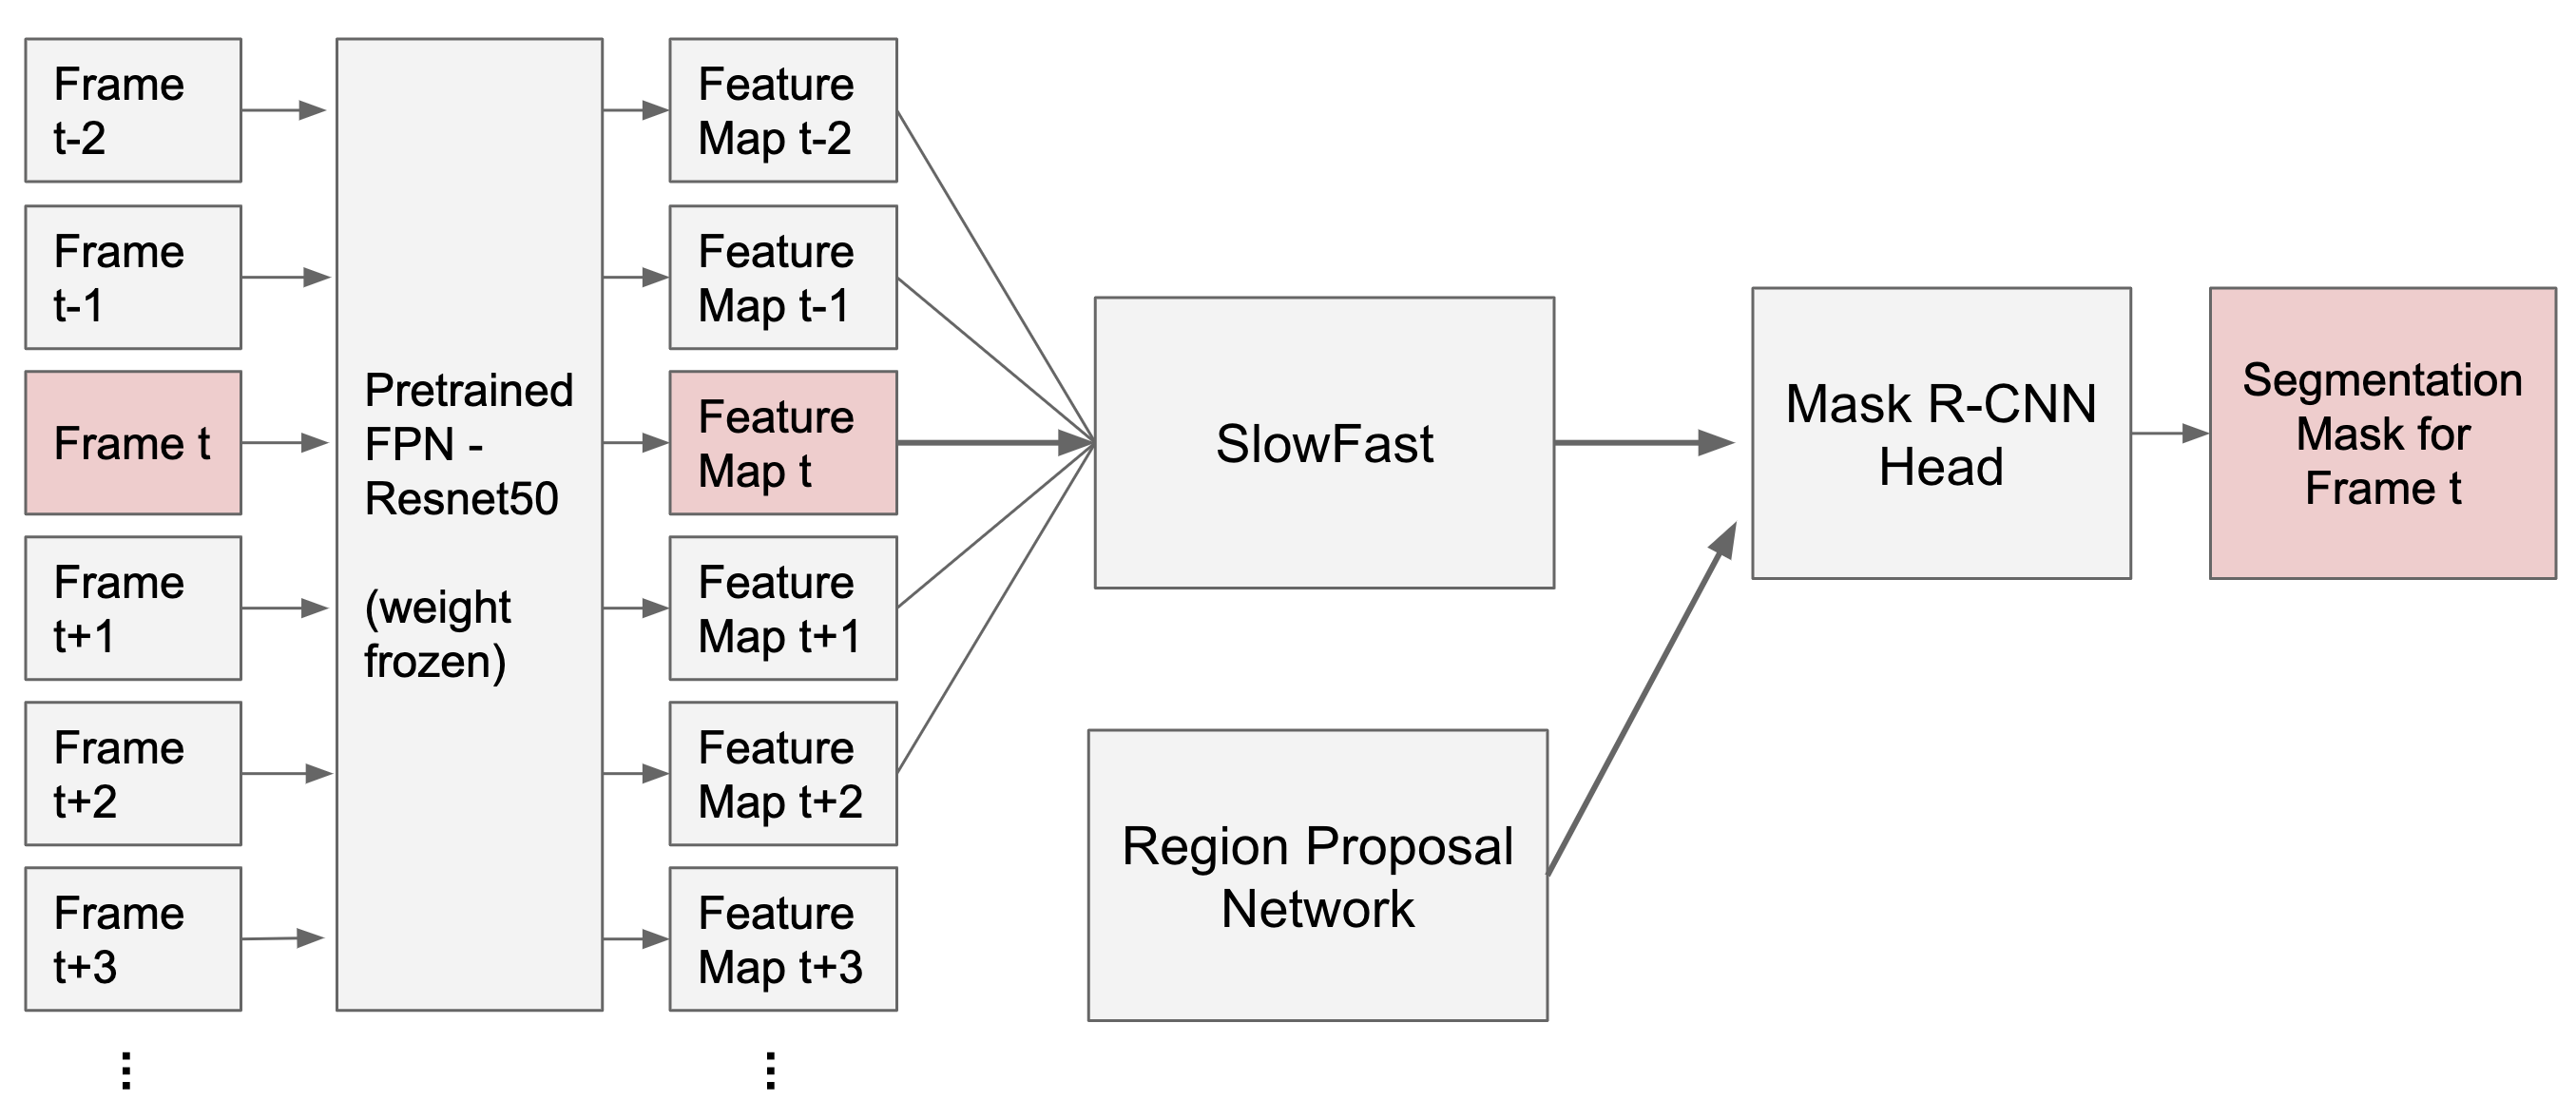
\includegraphics[width=\columnwidth]{figures/architecture.png}
	\caption{Architecture Overview.}
	\label{architecture}
\end{figure}

\begin{figure}
	\centering
	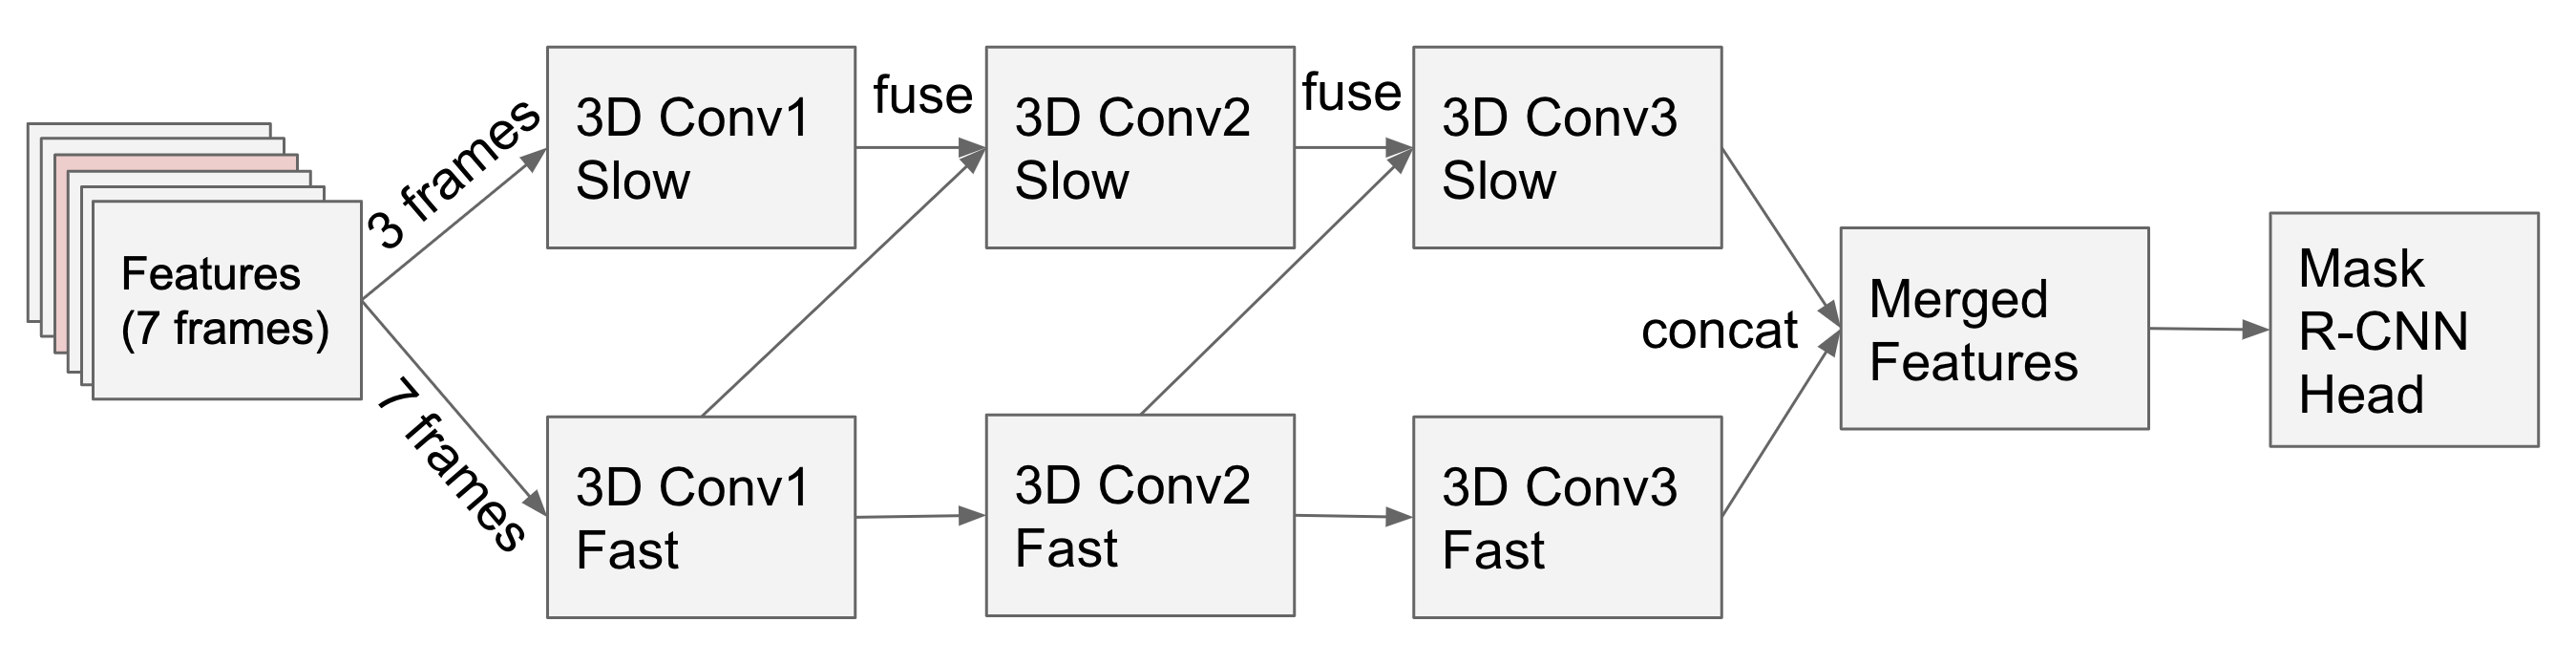
\includegraphics[width=\columnwidth]{figures/slowfast.png}
	\caption{Overview of SlowFast Layers.}
	\label{slowfast}
\end{figure}
\subsection{Training}
For the unsupervised case we are training for 20 epochs on the training data of DAVIS17 \cite{davis_2017}. We are using SGD with momentum as optimizer and our learning rate is set to 0.001. The semi-supervised training starts with a parent model trained on the task of unsupervised VOS and finetunes this model for 2000 iterations on the first frame for each sequence. We are using different augmentations, including Random Horizontal Flip, Rotation of up to 30 degrees, and Scaling of the image.